\subsection{Stylized facts, state count, and the spectral diagnostic}
\label{sec:res_stylized}

All three Cont stylized facts hold on both SPY windows (Figure~\ref{fig:stylized_facts}; Table~\ref{tab:model_comparison}, Observed row): the marginal is heavy-tailed (in-sample excess kurtosis $7.68$, out-of-sample $5.29$), linear autocorrelation in the raw growth rate is negligible, and volatility clustering in $|G_t|$ is persistent. A stationary block bootstrap at mean block length $20$ gives broadly overlapping IS and OoS $95\%$ CIs of $[2.17, 12.40]$ and $[0.90, 8.26]$ on the excess-kurtosis point estimates, so kurtosis targets should be read against the joint envelope rather than the points. Sweeping $K \in \{3, 6, 9, 12, 15, 18, 21\}$ for CHMM-N on the IS window, the $K = 3$ versus $K = 6$ comparison could not be separated under four-fold and six-fold rolling-origin cross-validation (mean held-out log-likelihood differences of $0.007$ and $0.027$ nats per observation, flipping sign between fold designs); with only four or six fold differences we treat these comparisons as descriptive. BIC and CAIC selected $K = 3$, and we chose $K^\star = 3$ as a parsimony choice, while $K = 18$ had a substantially lower mean held-out log-likelihood at both cadences. Absolute growth-rate ACF-MAE was nearly flat across the whole sweep, consistent with equation~\eqref{eq:acf_normalised}: a direct effective-rank diagnostic showed a single non-unit eigenvalue carrying $93.6\%$ of the lag-1 $|G|$ ACF at $K = 18$ on SPY, so the $K - 1$ rank bound did not bind at $K \ge 3$ on this instance. Repeating the diagnostic on the 30-ticker cross-section gave a wider distribution, with cross-ticker median dominant-mode share $0.76$ and minimum $0.326$ (NEM); the rank-non-binding claim is supported at the cross-ticker median rather than as a universal property of equity-return data.

\begin{figure}[t]
\centering
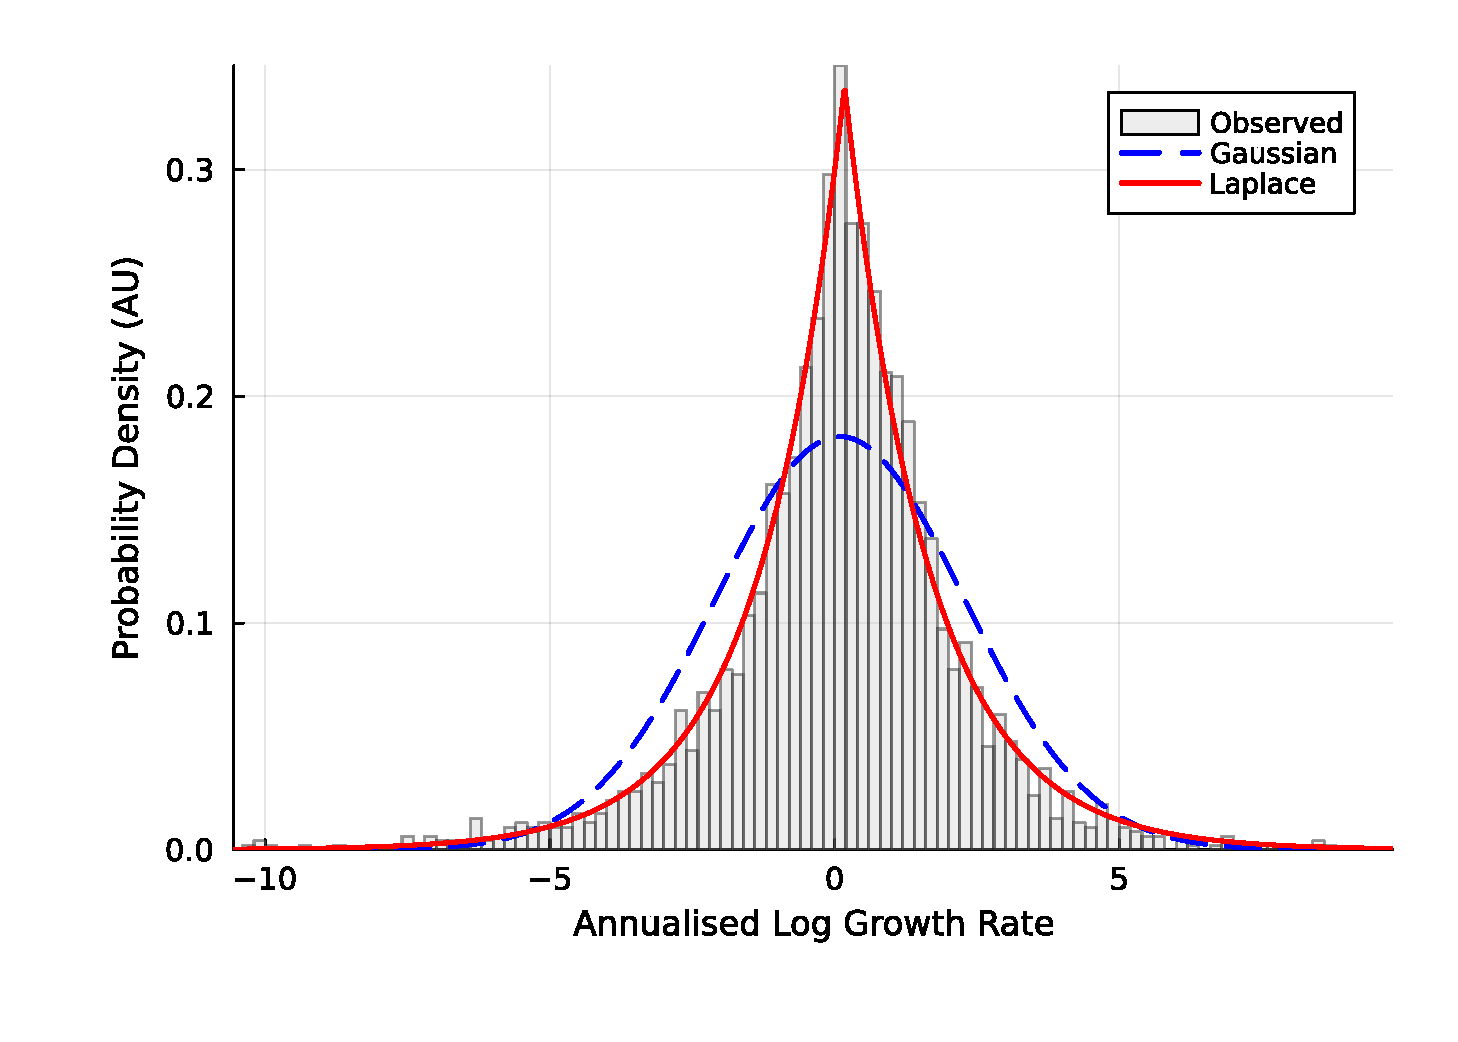
\includegraphics[width=0.49\columnwidth]{figs/Fig-1-Stylized-Facts-a.pdf}\hfill
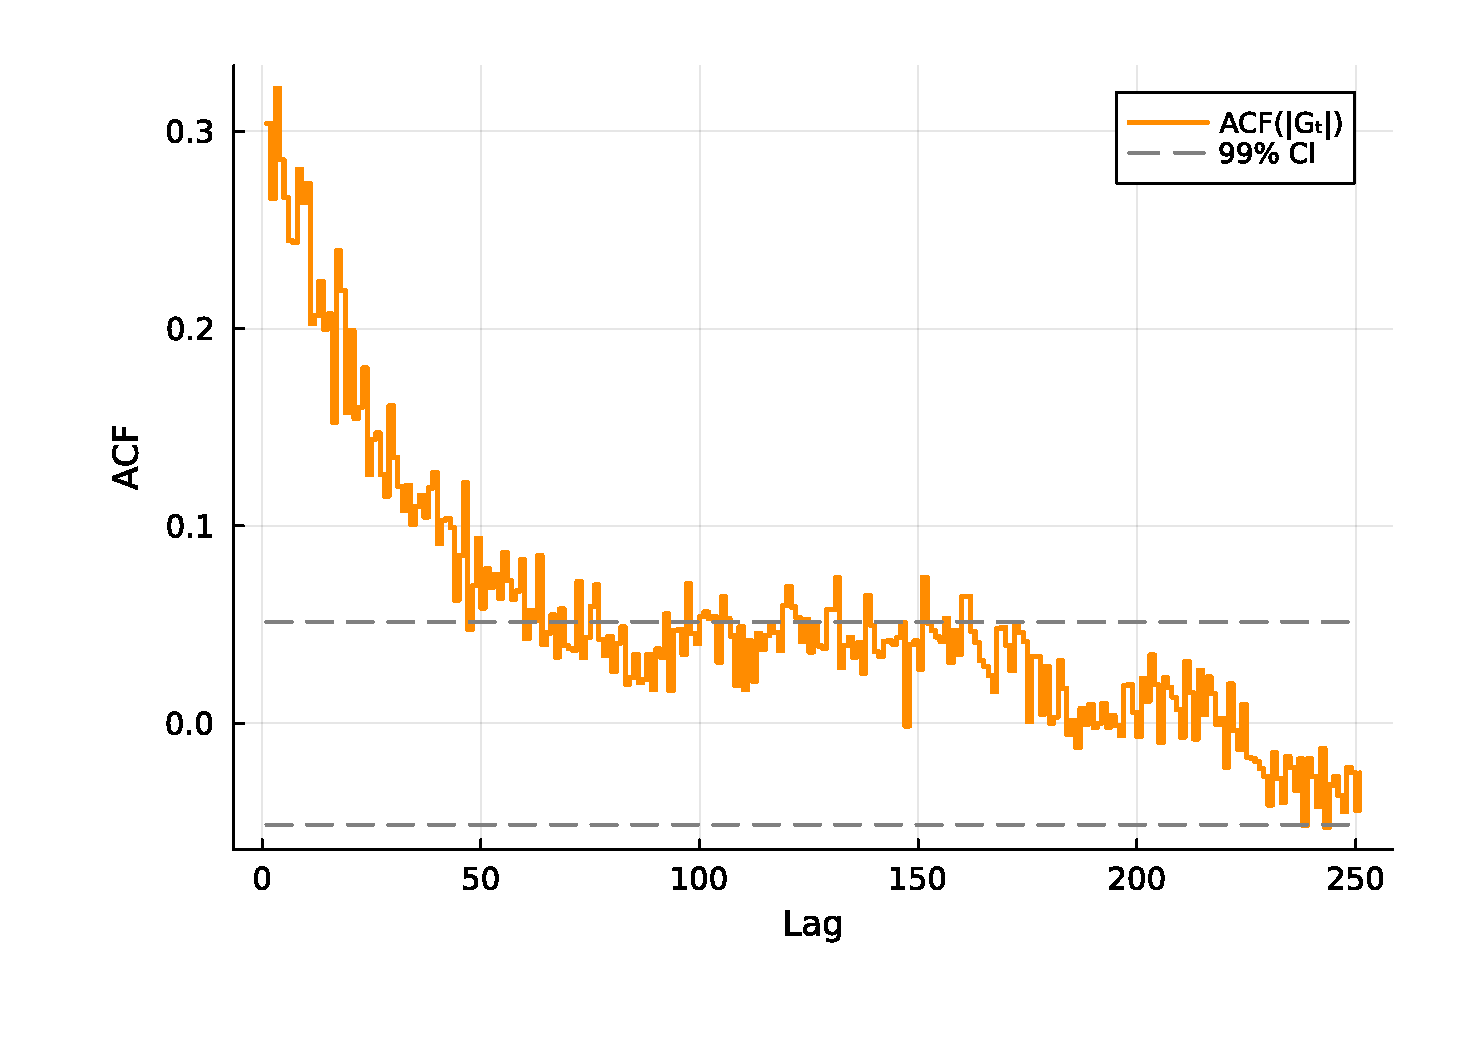
\includegraphics[width=0.49\columnwidth]{figs/Fig-1-Stylized-Facts-d.pdf}
\caption{The two channels of the low-$K$ Gaussian limitation on SPY. Left: heavy-tailed marginal of daily growth rates against Gaussian and Laplace fits (distributional channel). Right: slow decay of the absolute growth-rate ACF (temporal channel).}
\label{fig:stylized_facts}
\end{figure}

\subsection{Generator comparison}
\label{sec:res_generators}

With the state count fixed, we fit the four CHMM variants on the SPY IS window at $K^\star = 3$ and score them against the benchmark generators (Table~\ref{tab:model_comparison}). CHMM-N lands at $91.5\%$ IS and $78.0\%$ OoS KS, simulated excess kurtosis $3.83$ and $3.62$, and $|G_t|$ ACF-MAE $0.0462$ (on par with GARCH at $0.0490$). The shared-$\nu$ Student-$t$ provides the preferred marginal-fit and heavy-tail trade-off, the best CHMM OoS KS together with a smaller kurtosis gap than CHMM-N and no penalty hyperparameter, at $91.9\%$ IS and $82.1\%$ OoS KS with simulated excess kurtosis $4.68$ and $4.46$ against observed $7.68$ and $5.29$; on the kurtosis distance alone the penalty-free CHMM-L and CHMM-GED rows sit closer to observed, at lower KS. (A penalised per-state CHMM-t at $\lambda = 20$, with $\lambda$ tuned at $K = 18$ and re-used at $K^\star = 3$, overshot to IS excess kurtosis $18.87$ through a $1/\nu_k$-shrinkage artefact and is treated as a sensitivity reference only.) The four CHMM variants are statistically indistinguishable on OoS sample-CRPS (from $1.0393$ for CHMM-N to $1.0432$ for CHMM-L, against $1.0398$ for the bootstrap and $1.0440$ for GARCH(1,1)), so the family choice is driven by the per-row kurtosis match. The fitted CHMM matches the slow absolute growth-rate ACF within our lag-252 MAE tolerance on the SPY 2014--2024 instance, where the Ryd\'{e}n et al.~\cite{ryden1998stylized} $K = 2$ to $3$ Gaussian setup judged the ACF fit unsatisfactory, and the raw growth-rate ACF-MAE closes the negligible-linear-autocorrelation fact at $0.0235$ to $0.0240$, indistinguishable from the i.i.d.\ baselines. MS-GARCH stays well below the CHMM on KS under both point-estimate and Bayesian posterior-predictive variants, and the QuantGAN negative control fails all three stylized facts at this sample size ($0.0\%$ KS, excess kurtosis $0.56$, ACF-MAE at the i.i.d.\ floor).

\begin{table}[t]
\centering
\caption{Main generator comparison on SPY: $1{,}000$ simulated paths; IS $T = 2{,}516$, OoS $T = 572$. KS = Kolmogorov--Smirnov pass rate at $\alpha = 0.05$; Kurt = mean simulated excess kurtosis (observed $7.68$ IS, $5.29$ OoS); ACF-MAE over $252$ lags for absolute ($|G_t|$) and raw ($G_t$) growth rates. QuantGAN is the deep-generative negative control; the shared-$\nu$ CHMM-t fits a single $\nu$ across states with no penalty.}
\label{tab:model_comparison}
\footnotesize
\setlength{\tabcolsep}{3.4pt}
\renewcommand{\arraystretch}{0.97}
\begin{tabular}{l cc cc cc}
\toprule
& \multicolumn{2}{c}{KS (\%) $\uparrow$} & \multicolumn{2}{c}{Exc.\ Kurt} & \multicolumn{2}{c}{ACF-MAE $\downarrow$} \\
\cmidrule(lr){2-3} \cmidrule(lr){4-5} \cmidrule(lr){6-7}
Model & IS & OoS & IS & OoS & $|G_t|$ & $G_t$ \\
\midrule
\textit{Observed}     & --     & --     & $7.68$  & $5.29$  & --       & --       \\
Bootstrap             & $99.8$ & $91.8$ & $7.55$  & $6.86$  & $0.0628$ & $0.0235$ \\
GARCH(1,1)            & $27.4$ & $59.6$ & $7.59$  & $2.70$  & $0.0490$ & $0.0244$ \\
GARCH(1,1)-$t$        & $57.3$ & $80.8$ & $15.13$ & --      & $0.0316$ & $0.0173$ \\
MS-GARCH ($K=3$)      & $36.1$ & $33.1$ & $4.10$  & --      & $0.0284$ & $0.0173$ \\
QuantGAN TCN          & $0.0$  & $0.0$  & $0.56$  & $0.53$  & $0.0617$ & $0.0264$ \\
\midrule
CHMM-N                & $91.5$ & $78.0$ & $3.83$  & $3.62$  & $0.0462$ & $0.0240$ \\
CHMM-L                & $80.5$ & $63.6$ & $5.24$  & $5.20$  & $0.0530$ & $0.0235$ \\
CHMM-GED              & $90.3$ & $78.4$ & $5.45$  & $5.09$  & $0.0531$ & $0.0236$ \\
CHMM-t shared-$\nu$   & $91.9$ & $82.1$ & $4.68$  & $4.46$  & $0.0531$ & $0.0236$ \\
\midrule
ML HSMM-N             & $98.4$ & $91.0$ & $3.46$  & $3.38$  & $0.0629$ & $0.0236$ \\
\bottomrule
\end{tabular}
\end{table}

Two benchmark rows beat the CHMM on raw single-window OoS KS: the i.i.d.\ bootstrap ($91.8\%$) and the maximum-likelihood HSMM-N ($91.0\%$). That advantage is confined to the marginal axis: on volatility clustering both rows sit at the i.i.d.\ $|G_t|$ ACF-MAE floor ($0.0628$ and $0.0629$), while CHMM-N clusters below the floor at $0.0462$. The CHMM is the one generator in the panel equipped here with the regime-conditional VaR head: the i.i.d.\ bootstrap is structurally unable to produce a regime-conditional VaR (it carries no latent state), and HSMM-based risk heads are left as a companion-paper direction. A six-fold rolling-origin walk-forward reaches median OoS KS $62.1\%$ at $K^\star = 3$, with two stress folds (W2 COVID, W4 2022 rate-hike onset) below $10\%$ at both tested state counts ($K \in \{3, 18\}$, CHMM-N); we treat the walk-forward median, not the single-window OoS pair, as the right summary for judging live use.

\subsection{Tail index}
\label{sec:res_tail}

Because excess kurtosis is a fragile fourth-moment functional under heavy tails, we complement it with a threshold-local Hill estimate~\cite{hill1975tail} applied identically to the observed series and every simulated family at $K^\star = 3$ (top $5\%$ of $|G_t|$ exceedances); for the light-tailed mixture families this quantity is a shape diagnostic of the estimated threshold range, not an asymptotic tail index. The observed tail index is $\hat\alpha = 3.15$ IS and $3.30$ OoS, inside the $(2, 5)$ band reported by Cont~\cite{cont2001empirical} for daily equity returns, with a block-bootstrap $95\%$ CI of $[2.45, 4.25]$ on the IS estimate. The shared-$\nu$ CHMM-t lands at $\hat\alpha = 3.67$ on both windows with an across-path $95\%$ band of $[3.11, 4.38]$ overlapping the observed CI, so the simulated tail is matched, sitting slightly thinner in the far tail, rather than undershot. Every emission family produces an in-band estimate at $K^\star = 3$ (CHMM-N $3.41$, CHMM-L $3.26$, CHMM-GED $3.24$) even though simulated excess kurtosis spans $3.83$ to $18.87$ across the same rows: at the depths the estimator sees, the regime mixture rather than the emission family carries the heavy tail, while the emission shape governs how far into the extreme tail the match extends. Applied per tail side, the same estimator reproduces the direction of the observed gain/loss asymmetry (observed loss-minus-gain gap $-0.55$; shared-$\nu$ $-0.46$, CHMM-L $-0.44$) from the regime means alone.

\subsection{Cross-ticker generalisation and refit}
\label{sec:res_crossticker}

Fitting one model per ticker on the sector-balanced 30-ticker panel, the in-sample KS distribution is concentrated (median $96.8\%$) and the out-of-sample distribution is wider, with median $69.1\%$, mean $66.2 \pm 28.2\%$, and $11/30$ tickers below $60\%$. The deepest failures are tickers that introduced a new regime out of sample: LLY and UNH in Health Care, NEM in Materials. An ANOVA on OoS KS by sector returned no significant sector effect on either the original $n = 3$ design or an $n = 6$ expansion to a 60-ticker panel, so the visible concentration of failures on regime-introducing tickers is a per-ticker observation rather than evidence of sector-level structure. Periodic refit closes much of the gap: at $K^\star = 3$ a quarterly refit shifts the OoS KS median from $69.1\%$ to $84.7\%$ and reduces failures from $11/30$ to $8/30$. In companion multi-asset experiments, per-asset CHMM marginals compose through a rank-based Student-$t$ copula that reproduces contemporaneous cross-asset correlations (in-sample off-diagonal MAE $0.027$ on a six-asset basket); that construction is cross-sectional only, preserving each asset's marginal and the contemporaneous dependence but not per-asset serial dependence, and is not evaluated further here.

\subsection{Regime-conditional Value-at-Risk}
\label{sec:res_var}

We back-test a regime-conditional VaR built from the CHMM one-step-ahead state forecast: the forward filter runs under IS-fixed parameters $(\mathbf T, \{\boldsymbol\theta_k\})$, only the one-step-ahead state-probability vector updates through the OoS window, and the VaR is the $\alpha$-quantile of the state-mixture predictive. The back-test covers all $573$ held-out forecasts (Table~\ref{tab:cond_var}). At VaR level $\alpha = 0.05$ the CHMM rows are not rejected by Christoffersen-cc ($p_{\text{cc}} \in [0.39, 0.67]$ across CHMM configurations), and CHMM-N at $K^\star = 3$ is likewise not rejected by the DQ test ($p = 0.09$); non-rejection at these sample sizes indicates compatibility with correct conditional coverage rather than a demonstration of it. Breach rates at $\alpha = 0.05$ sit close to nominal, from $26$ breaches ($4.54\%$) at $K = 18$ to $36$ ($6.28\%$) at $K^\star = 3$, and no CHMM row is rejected by Kupiec or Christoffersen-ind at that level. The $\alpha = 0.01$ rows are also not rejected by Christoffersen-cc ($p_{\text{cc}} \in [0.10, 0.16]$) but are power-bounded at $\TOoS{573}$, where only about $5.7$ breaches are expected; the higher-power DQ test separates the state counts, rejecting CHMM-N at $K = 18$ ($p = 0.02$) while $K^\star = 3$ escapes rejection only marginally ($p = 0.06$). Against the two non-state-space contenders the CHMM rows reach approximate parity at $\alpha = 0.05$; at $\alpha = 0.01$ only CHMM-N at $K^\star = 3$ is not rejected by DQ, a power-bounded non-rejection rather than evidence of a significant difference, since failure to reject does not establish the null and no pairwise model-comparison test was conducted. The filtered bootstrap ($p = 0.04$) and CAViaR ($p = 0.01$) are both rejected at that tier, as is every other CHMM family and state count in the full sixteen-row family panel of the extended experiments ($p$ from $0.0005$ to $0.030$). Extending to six rolling-origin walk-forward folds, Christoffersen-cc does not reject on $19$ of $24$ rows at the $5\%$ test level, with the five rejections concentrated on stress folds: all four W2 (COVID 2020) rows reject, while W4 (2022 rate-hike onset) produces a single tail-tier rejection at $K = 18$, $\alpha = 0.01$; we read these multi-row panels as multiplicity-aware descriptive evidence rather than repeated confirmations.

\begin{table}[t]
\centering
\caption{Regime-conditional VaR back-test on SPY OoS ($\TOoS{573}$ forecasts including the boundary return; seed fixed). CHMM rows use the forward filter under IS-fixed parameters; contenders are scored on the same Christoffersen/DQ harness. $\alpha = 0.01$ rows are power-bounded at this sample size; DQ $p$-values use the 4-lag specification.}
\label{tab:cond_var}
\footnotesize
\setlength{\tabcolsep}{5pt}
\begin{tabular}{l c c c c c c}
\toprule
Model & $K$ & $\alpha$ & Breaches & Rate & $p_{\text{cc}}$ & $p_{\text{DQ}}$ \\
\midrule
CHMM-N             & $3$  & $0.01$ & $9$  & $1.57\%$ & $0.14$ & $0.06$ \\
CHMM-N             & $3$  & $0.05$ & $36$ & $6.28\%$ & $0.39$ & $0.09$ \\
CHMM-N             & $18$ & $0.01$ & $9$  & $1.57\%$ & $0.14$ & $0.02$ \\
CHMM-N             & $18$ & $0.05$ & $26$ & $4.54\%$ & $0.67$ & $0.68$ \\
\midrule
Filtered bootstrap & --   & $0.01$ & $8$  & $1.40\%$ & $0.16$ & $0.04$ \\
Filtered bootstrap & --   & $0.05$ & $24$ & $4.19\%$ & $0.43$ & $0.55$ \\
CAViaR (SAV)       & --   & $0.01$ & $6$  & $1.05\%$ & $0.14$ & $0.01$ \\
CAViaR (SAV)       & --   & $0.05$ & $25$ & $4.36\%$ & $0.55$ & $0.76$ \\
\bottomrule
\end{tabular}
\end{table}
